\documentclass[a4paper,12pt]{book}


%************
%* packages *
%************


\usepackage[latin1]{inputenc}
\usepackage[italian]{babel}
\usepackage{fancyhdr}
\usepackage{verbatim}
\usepackage{float}
\usepackage{subfigure}
\usepackage[stable]{footmisc}
\usepackage[hang,small,sf]{caption}
\usepackage{cite}
\usepackage{acronym}
\usepackage{sectsty}
\usepackage{listings}
\usepackage[usenames]{color}
\usepackage{graphicx}
\usepackage[italian]{varioref}
\usepackage{lmodern}
\usepackage[left=2.5cm,right=2.5cm,bottom=2.8cm]{geometry}
\usepackage{colortbl}
\usepackage{booktabs,graphicx,pgfgantt,tikz-uml}
\usepackage{fontspec}
\usetikzlibrary{shapes,arrows,chains}
\usepackage{acronym}


%*****************
%* nuovi comandi *
%*****************

\newcommand{\abs}[1]{\left|#1\right|}                               % modulo
\newcommand{\dato}{\left|\right.}                                   % probabilit\`{a} condizionata
\newcommand{\fun}[1]{\mathrm{#1}}                                   % stile funzione
\newcommand{\imp}{\;\;\Longrightarrow\;\;}                          % implicazione
\newcommand{\norma}[1]{\left\| #1 \right\|}                         % norma
\newcommand{\prob}[1]{\mathrm{P}\!\left[#1\right]}                  % probabilit\`{a}
\newcommand{\expect}[1]{\mathrm{E}\!\left[#1\right]}                % aspettazione
\newcommand{\sse}{\;\;\Longleftrightarrow\;\;}                      % se e solo se
\newcommand{\vect}[1]{{\boldsymbol{\mathrm{#1}}}}                   % stile vettore
\newcommand{\real}[1]{\fun{Re}\left[#1\right]}                      % parte reale
\newcommand{\imag}[1]{\fun{Im}\left[#1\right]}                      % parte immaginaria
\newcommand{\Dim}[1]{\fun{dim}\left[#1\right]}                      % dimensione di una matrice
\newcommand{\Det}[1]{\fun{det}\left[#1\right]}                      % determinante di una matrice
\newcommand{\Ker}[1]{\fun{ker}\left[#1\right]}                      % ker di una matrice
\newcommand{\rango}[1]{\fun{rango}\left[#1\right]}                  % rango di una matrice
\newcommand{\scalare}[2]{\left\langle #1, #2 \right\rangle}         % prodotto scalare
\newcommand{\blbrace}{\left  \lbrace}                               % parentesi graffa sinistra grande
\newcommand{\brbrace}{\right \rbrace}                               % parentesi graffa destra grande
\newcommand{\sinc}{\fun{sinc}}                                      % sinc
\newcommand{\rect}{\fun{rect}}                                      % rect
\newcommand{\rcos}{\fun{rcos}}                                      % rcos
\newcommand{\sgn}{\fun{sgn}}                                        % sgn
\newcommand{\N}{\mathbb{N}}                                         % insieme dei numeri naturali
\newcommand{\Z}{\mathbb{Z}}                                         % insieme dei numeri interi
\newcommand{\Q}{\mathbb{Q}}                                         % insieme dei numeri razionali
\newcommand{\R}{\mathbb{R}}                                         % insieme dei numeri reali
\newcommand{\C}{\mathbb{C}}                                         % insieme dei numeri complessi
\newcommand{\seq}[2][n]{#2_{0}, #2_{1}, \ldots, \, #2_{#1}}         % sequenza
\newcommand{\Span}[2][n]
{\fun{span} \blbrace #2_{1}, #2_{2}, \ldots, \, #2_{#1} \brbrace}   % spazio generato
\newcommand{\ddt}{\frac{\fun{d}}{\fun{dt}}}                         % derivata
\newcommand{\Div}[2]{#1 \; \mid \; #2}                              % divide
\newcommand{\MCD}[2]{\fun{MCD}\(#1, #2\)}                           % massimo comun divisore
\newcommand{\mcm}[2]{\fun{mcm}\(#1, #2\)}                           % minimo comune multiplo
\newcommand{\goodgap}{
                      \hspace{\subfigtopskip}
                      \hspace{\subfigbottomskip}
                     }                                              % interlinea opportuna per le sottofigure
\newcommand{\eng}[1]{\emph{#1}}                                   % inglese
\newcommand{\virg}[1]{``#1"}                                        % fa una citazione tra virgolette
%\newcommand{\unit}[2]($\frac{\text{#1}}{\text{#2}}$)                % unit\`{a} di misura
\newcommand{\textttvar}[1]{{\ttvar #1}}

\definecolor{gray}{gray}{0.9}
\newcommand{\listato}[1]{\lstset{language=#1, numbers=left, numberstyle=\tiny, stepnumber=2, numbersep=5pt, numberblanklines=false, xleftmargin=5pt, captionpos=b, stringstyle=\ttfamily, columns=flexible, showstringspaces=false, tabsize=2, frame=single, framerule=0pt, backgroundcolor=\color{gray}, basicstyle=\small}}

%****************************
%* ridefinizioni di comandi *
%****************************

\renewcommand{\(}{\left(}                                     % parentesi tonda sinistra grande
\renewcommand{\)}{\right)}                                    % parentesi tonda destra grande
\renewcommand{\[}{\left[}                                     % parentesi quadra sinistra grande
\renewcommand{\]}{\right]}                                    % parentesi quadra destra grande
\renewcommand{\exp}[1]{\fun{e}^{#1}}                          % esponenziale
\renewcommand{\gcd}[2]{\fun{gcd}\(#1, #2\)}                   % massimo comun divisore

\renewcommand{\lstlistingname}{Codice}
\renewcommand{\lstlistlistingname}{Elenco dei listati codice}

\newfont{\ttvar}{cmvtt10 scaled 1200}     % nuovo carattere tipi courier a spaziatura variabile per le dimostrazioni


% interlinea
%\renewcommand{\baselinestretch}{1.25}

% margini
%\setlength{\topmargin}{-1cm}
%\setlength{\textheight}{24cm}
%\setlength{\textwidth}{17cm}
%\setlength{\oddsidemargin}{-0.6cm}
%\setlength{\evensidemargin}{-0.6cm}
%\setlength{\headsep}{1.0cm}
%\setlength{\footskip}{1.0cm}
%\setlength{\parindent}{0.7cm}
%\setlength{\captionmargin}{0.7cm}

% margini senato
\textwidth       =  14.50 cm            % larghezza 21 cm - 4 cm (sinistro) - 2.5 (destro)
\textheight      =  23.10 cm            % altezza 29.7 cm - 3 cm (superiore) - 2 (inferiore)
\topmargin       =   0.00 cm            % margine superiore 3 cm diminuito di 1 inch
\oddsidemargin   =   1.46 cm            % margine sinistro 4 cm diminuito di 1 inch
\evensidemargin  =  -0.04 cm            % margine destro 2.5 cm diminuito di un inch
%\renewcommand{\baselinestretch}{1.25}   % interlinea
\setlength{\headsep}{1.0cm}
\setlength{\footskip}{1.0cm}
\parindent = 0.7cm
\captionmargin = 0.7cm



% stile pagina
\pagestyle{fancy}
\renewcommand{\chaptermark}[1]{\markboth{\chaptername\ \thechapter.\ #1 }{}}
\renewcommand{\sectionmark}[1]{\markright{\thesection\ #1}{}}
\fancyhead{}
\fancyhead[LE,RO]{\sffamily \thepage}
\fancyhead[RE]{\sffamily \leftmark}
\fancyhead[LO]{\sffamily \rightmark}
\fancyfoot{}

% ridefinisco lo stile plain
\fancypagestyle{plain}{ \fancyhead{} \fancyfoot{}
\fancyfoot[C]{\sffamily \thepage}
\renewcommand{\headrulewidth}{0pt}}

% stile per i titoli
\allsectionsfont{\sffamily \raggedright}

% definisco i colori
\definecolor{light_yellow}{rgb}{1,1,0.7}
\definecolor{dark_yellow}{rgb}{1,1,0.5}
\definecolor{my_green}{rgb}{0,0.6,0}
\definecolor{my_red}{rgb}{0.8,0,0}

% definisco il codice sql
\lstset{basicstyle=\small\ttfamily,language=SQL, keywordstyle=\color{blue},commentstyle=\color{blue}, stringstyle=\color{my_green}}

\usepackage{xcolor}

\colorlet{punct}{red!60!black}
\definecolor{background}{HTML}{FFFCEE}
\definecolor{table}{HTML}{CCCCCC}
\definecolor{delim}{RGB}{20,105,176}
\colorlet{numb}{green!60!black}

\lstdefinelanguage{json}{
    basicstyle=\normalfont\ttfamily,
    numbers=left,
    numberstyle=\scriptsize,
    stepnumber=1,
    numbersep=8pt,
    showstringspaces=false,
    breaklines=true,
    frame=lines,
    backgroundcolor=\color{background},
    stringstyle=\color{red}\ttfamily,
    morestring=[b]',
    morestring=[b]",
    literate=
     *{0}{{{\color{numb}0}}}{1}
      {1}{{{\color{numb}1}}}{1}
      {2}{{{\color{numb}2}}}{1}
      {3}{{{\color{numb}3}}}{1}
      {4}{{{\color{numb}4}}}{1}
      {5}{{{\color{numb}5}}}{1}
      {6}{{{\color{numb}6}}}{1}
      {7}{{{\color{numb}7}}}{1}
      {8}{{{\color{numb}8}}}{1}
      {9}{{{\color{numb}9}}}{1}
      {:}{{{\color{punct}{:}}}}{1}
      {,}{{{\color{punct}{,}}}}{1}
      {\{}{{{\color{delim}{\{}}}}{1}
      {\}}{{{\color{delim}{\}}}}}{1}
      {[}{{{\color{delim}{[}}}}{1}
      {]}{{{\color{delim}{]}}}}{1}
}
\lstset{numbers=left, numberstyle=\scriptsize, stepnumber=1, numbersep=5pt,
    xleftmargin=3.0ex}
\lstdefinelanguage{JavaScript}{
  backgroundcolor=\color{background},
  frame=lines,
  basicstyle=\ttfamily\footnotesize,
  keywords={typeof, new, true, false, catch, function, return, null, catch,%
  switch, default, var, if, in, while, do, else, case, break},
  keywordstyle=\color{blue}\bfseries, ndkeywords={class, export, boolean, throw, implements, import, this},
  ndkeywordstyle=\color{darkgray}\bfseries,
  identifierstyle=\color{black},
  sensitive=false,
  comment=[l]{//},
  morecomment=[s]{/*}{*/},
  commentstyle=\color{purple}\ttfamily,
  stringstyle=\color{red}\ttfamily,
  morestring=[b]',
  morestring=[b]"
} 





\begin{document}

\begin{titlepage}
\begin{center}
% Upper part of the page. The '~' is needed because \\
% only works if a paragraph has started.

\includegraphics[scale=0.08]{logo.png}\\[1.5cm]
\textsc{\LARGE Università degli Studi di Padova}\\[1.2cm]
\textsc{\Large Dipartimento di Ingegneria dell'Informazione}\\[0.8cm]
\textsc{\Large Corso di Laurea Triennale in}\\[0.5cm]
\textsc{\Large Ingegneria Informatica}\\[2cm]
% Title
{ \LARGE \bfseries Applicazione per l'indagine sulla soddisfazione dei
clienti}\\[1cm]
{  \bfseries Customer satisfaction survey application}\\[2cm] 
\textsc{\large Relatore: Prof.~Giorgio~Maria~Di~Nunzio}\\[0.5cm]
\textsc{\large Laureando: Alex~Tomasello}\\
\vfill
% Bottom of the page
{\large Anno Accademico 2012/2013}
\end{center}
\end{titlepage}


\thispagestyle{empty} % pagina bianca dopo il titolo
\cleardoublepage


\pagenumbering{roman} % numerazione romana per gli indici
\thispagestyle{empty}

\clearpage{\pagestyle{plain}\cleardoublepage}
\tableofcontents


\clearpage{\pagestyle{plain}\cleardoublepage} % numerazione arabica per i capitoli
\pagenumbering{arabic}

%\clearpage{\pagestyle{plain}\cleardoublepage}
%\chapter*{Sommario}
%\addcontentsline{toc}{chapter}{Sommario}
%\input{sommario}


\clearpage{\pagestyle{plain}\cleardoublepage}
\chapter{Introduzione}
\section{Introduzione}
A partire dagli anni novanta del XX secolo la tecnologia, lo sviluppo e la
competizione nel mercato hanno portato le grandi aziende, soprattutto operanti nel settore
terziaro del lavoro, ad avere la necessità di monitorare la qualità dei loro
servizi. 
La scelta di un approccio di mercato del tipo \textit{customer
oriented} rende necessaria l'effettuazione di indagini interne
mirate a monitorare il \textit{modus operandi} dei dipendenti,la competenza,il clima di gruppo, le
risorse e le difficoltà. Di fondametale importanza risultano anche le verifiche
proposte per analizzare la soddisfazione e i bisogni dei clienti, al fine di
proporre nuovi servizi o per migliorare quelli già offerti, così da poter
continuare ad essere non solo competitivi nel mercato, ma leader nel settore al
quale appartengono. Permettere al cliente di esprimere un'opinione sulla qualità
dei servizi offerti, da' la possibilità di mettere in evidenza quali sono le
caratteristiche che fanno eccellere la ditta e favorisce l'individuazione degli
aspetti su cui bisogna investire risorse per migliorarli.

Al fine di cogliere e valutare il livello di soddisfazione è stato idealizzato
il modello \textit{SERVQUAL} (Parasuraman, Zeithaml e Berry). Il
\textit{SERVQUAL} è costituito da due serie di 22 domande predefinite alle quali
corrispondono delle risposte con valutazione numerica con scala da 1 a 7 ,
mettendo a confronto le aspettative generiche del cliente nei confronti del
servizio e la percezione del prodotto offerto.
Il modello  consente di misurare il CS per 5 elementi fondamentali del
servizio: 
\begin{itemize}
  \item \textbf{Elementi tangibili}: aspetto delle strutture fisiche,
  delle attrezzature e del personale;
  \item \textbf{Affidabilità}: capacità di erogare il servizio promesso
  in modo affidabile e preciso;
  \item \textbf{Capacità di risposta}: volontà di aiutare i clienti e di
  fornire il servizio con prontezza;
  \item \textbf{Capacità di rassicurazione} : competenza e cortesia
  degli impiegati e loro capacità di  ispirare fiducia e sicurezza;
  \item \textbf{Empatia} : assistenza premurosa e individualizzata che
  l’azienda riserva ai suoi clienti.
\end{itemize}

I risultati del confronto fra \textit{attese} (\textbf{A}) e \textit{percezioni}
(\textbf{P}) di qualità possono essere di tre tipi:
\begin{itemize}
  \item P > A : la qualità del servizio è molto alta perchè le
  percezioni superano le aspettative;
  \item P = A : la qualità del servizio è buona perchè si sono soddisfatte
  in pieno le attese del cliente;
  \item P < A : la qualità del servizio è bassa. Se P è
  molto vicino, cioè solo di poco inferiore ad A e queste ultime erano
  alte, il risultato deve essere considerato buono perchè si sono soddisfatte
  quasi del tutto le elevate attese di qualità del cliente. Questo è tanto
  più vero quanto più il servizio è complesso tecnicamente o sofisticato come
  immagine, ecc. Il risultato sarà, invece, negativo solo se P è abbastanza o
  molto inferiore ad A, per cui il cliente è abbastanza o molto deluso dalla
  qualità del servizio.
\end{itemize}

Durante il periodo di stage che ho sostenuto presso SAIV S.p.A.
in collaborazione con il tutor aziendale Lovato Giovanni e il collega Rigoni
Giulio , è stata sviluppata un'applicazione per monitorare 




\clearpage{\pagestyle{plain}\cleardoublepage}
\chapter{Descrizione del progetto}
\label{cha:descrizione}
 \section{Scelte progettuali}
Durante il periodo di stage che ho sostenuto presso SAIV S.p.A., in
collaborazione con il tutor aziendale dott. Lovato Giovanni e il collega Rigoni
Giulio , è stata sviluppata un'applicazione per monitorare il livello di CS.

Questa applicazione è stata creata a seguito di una reale richiesta di una
commessa da parte di un'azienda. L'Ente aveva richiesto uno strumento intuitivo
e veloce da affiancare al ServQual, in modo da facilitare anche i clienti che
ritenevano troppo impegnativa la compilazione del questionario, coinvolgere
quindi quanti più utenti possibili, avere una maggiore quantità di dati ed un
feedback immediato.

Per diritti di privacy aziendale sostituirò il nome del committente con
l'Università degli Studi di Padova e ho adattato l'applicazione finalizzandola a
monitorare i servizi offerti dalla segreteria studenti.

\section{Presentazione del modello}

La nostra applicazione è certamente più veloce ed intuitiva rispetto al modello
ServQual.
Altro punto di forza dell'applicazione è l'automatizzazione. A differenza del
questionario cartaceo in cui poi risulta necessario registrare i dati,
elaborarli ed archiviarli, l'applicazione permette queste operazioni in tempi
veloci e contemporaneamente all'espressione del voto da parte del cliente, in
modalità automatica.

E' necessario evidenziare che il nostro modello non è esaustivo. E'
un'applicazione da affiancare ad altri strumenti, è una modalità che permette di
avere un feedback generale e veloce, ma non completo. Per essere un modello
valido sarebbe necessario elaborarlo ulteriormente.

L'utente ha la possibilità di esprimere la propria valutazione scegliendo tra le
possibilità: non del tutto soddisfatto, mediamente soddisfatto e molto
soddisfatto. Ad ogni alternativa abbiamo conferito un valore: a ``non del tutto
soddisfatto'' il valore 1, a ``mediamente soddisfatto'' il valore 3, a ``molto
soddisfatto'' il valore 5. La scelta dei valori è stata fatta per permettere, in
un tempo successivo, l'inserimento di altre valutazioni intermedie (2 e 4) che
faciliterebbero una visione più completa.

All'utente sarà permesso di esprimere il proprio voto in modo anonimo,
intuitivo e veloce con la possibilità di aggiungere un commento che verrà registra-
to dal sistema. L'amministratore, invece, potrà analizzare i dati, anche in tempo
reale, visualizzati su grafici. Ad una prima analisi della commessa con il team, è stata
presa la decisione di realizzare un' applicazione con una sezione front end, otti-
mizzata per eseguita su dispositivi touchscreen e una sezione back end accessibile
solo dagli amministratori.
Nel momento in cui ci siamo chiesti quali dati sarebbe stato utile salvare,
abbiamo deciso di registrare nel sistema il commento, il nominativo e l'e-mail
dell'utente (dati presentati come facoltativi, con il modello per la privacy e
l'utilizzazione dei dati), la data di votazione in formato gg/mm/aa, il
department per gli sportelli di facoltà e lo score. Il commento personale
permetterà all'ente di avere un riscontro più completo rispetto alla singola
risposta di scelta multipla e molto utile al fine di una verifica dei servizi
proposti, il nome e l'indirizzo di posta elettronica consentiranno al
committente di contattare la persona che lo ha richiesto e la data di votazione
può facilitare l'analisi dell'affluenza al servizio.

\section{Casi d'uso}
Inserimento della votazione, lato \emph{front end}:
\begin{itemize}
  \item \textbf{Voto in uscita} : In uscita dalla segreteria lo studente
  troverà un totem multimediale touch screen con cui potrà esprimere il
  proprio livello di soddisfazione dopo aver usufruito dei servizi offerti. La
  schermata di introduzione è composta da un messaggio inserito per spiegare
  all'utilizzatore la finalità per la quale viene richiesto di lasciare un
  \emph{feedback}, un video introduttivo dell'Università degli Studi di Padova
  e la scelta dell'operazione effettuata : servizio ricevuto presso lo sportello
  di facoltà o sportello veloce (Figura~\ref{fig:scorecard}).
  \item \textbf{Inserimento commento} : Lo studente può lasciare un proprio
  commento selezionando l'area con la voce ``Laciaci un commento''. Comparirà un finestra di dialogo che permetterà
  l'inserimento del testo , il nome e cognome e l'indirizzo email se il cliente
  vuole essere contattato. Per registrare il commento bisogna accettare le
  condizioni sulla privacy~(Figura~\ref{fig:comment}).
  \item \textbf{Registrazione del voto} : Il cliente esprime il proprio livello
  di soddisfazione tramite l’interfaccia selezionando uno dei 3 bottoni. In caso l'utente avesse
  selezionato nella schermata precedente la voce ``servizio sportello di
  facoltà'' un menu a tendina comparirà per indicare lo sportello difacoltà al
  quale si è rivolto~(Figura~\ref{fig:voting}).
  \item \textbf{Feedback all'utente} : Terminato il processo di registrazione
  una finestra di dialogo certifica all'utente che il processo di voto si è
  concluso in modo corretto~(Figura~\ref{fig:stored}).
    \begin{figure}[!h]
    \begin{center}
        
\includegraphics[scale=0.32]{scorecard.png}
        \caption{Schermata introduttiva}
        \label{fig:scorecard}
    \end{center}
  \end{figure}
   \begin{figure}[!h]
    \begin{center}
        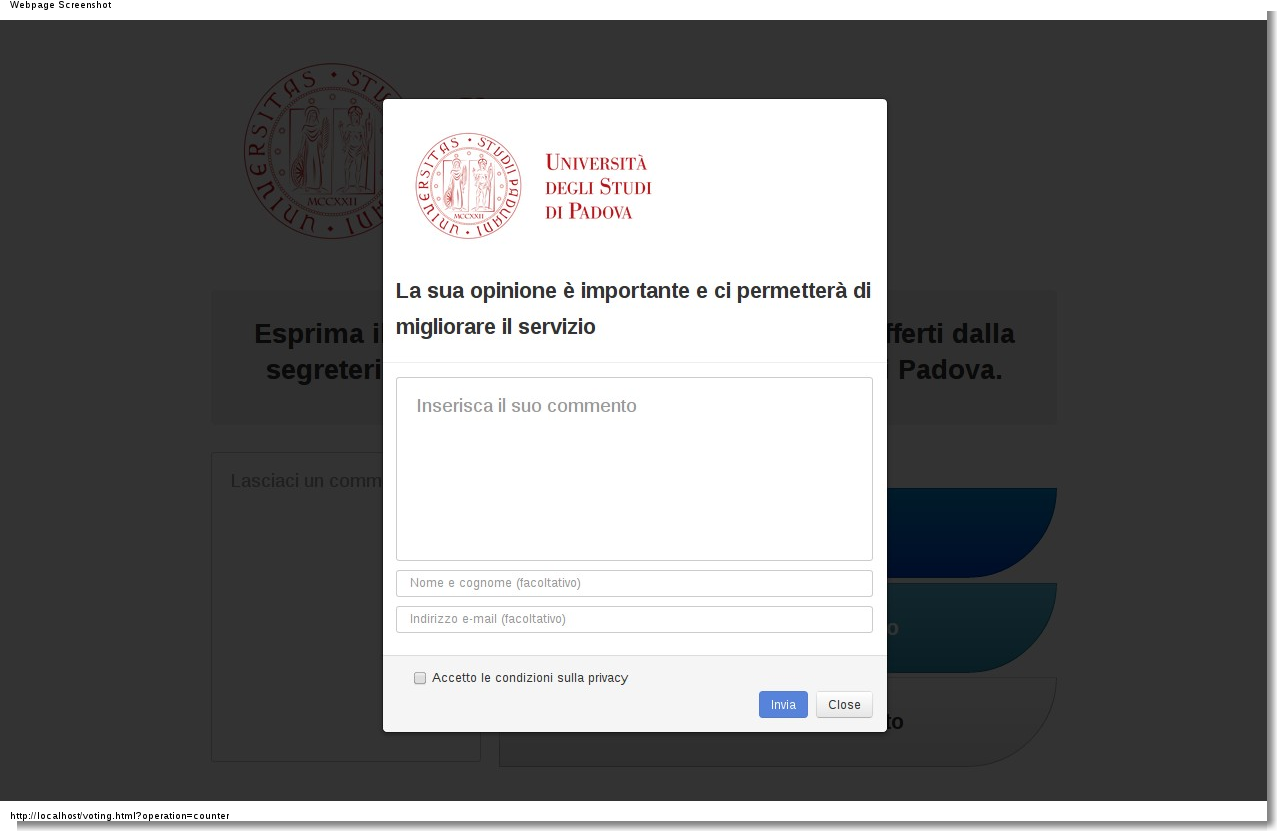
\includegraphics[scale=0.32]{comment.png}
        \caption{Inserimento di un commento}
        \label{fig:comment}
    \end{center}
  \end{figure}
   \begin{figure}[!h]
    \begin{center}
        
\includegraphics[scale=0.32]{voting.png}
        \caption{Scelta del livello di soddisfazione}
        \label{fig:voting}
    \end{center}
  \end{figure}
  \begin{figure}[!h]
    \begin{center}
        
\includegraphics[scale=0.32]{stored.png}
        \caption{Feedback all'utente}
        \label{fig:stored}
    \end{center}
  \end{figure}
\end{itemize}
\\\\
Consultazione dei voti \emph{back end}:Caso d’uso 2 (Consultazione dei voti). Un altro caso d’uso prevede la consultazione dell’andamento del livello di CS da parte
dell’Amministratore del Sistema (vedi Figura 2). L’Amministratore del Sistema potrà accedere via browser web a un’interfaccia
di consultazione dei voti, che presenterà in modo grafico l’andamento del livello di CS filiale per filiale.
1. L’Amministratore accede all’interfaccia web del Sistema.
2. Il Sistema genera i grafici relativi all’andamento della CS

\section{Classi}

\section{Strumentazione}
I linguaggi in cui verrà sviluppato il sistema sono HyperText Markup Language (HTML), Cascading Style Sheets (CSS) e
JavaScript (JS) con database di appoggio CouchDB, tramite i quali sarà implementata un’applicazione web aderendo al paradigma Model-View-Controller (MVC).

\clearpage{\pagestyle{plain}\cleardoublepage}
\chapter{CouchDB}
\label{cha:CouchDB}
\section{CouchDB}
\section{JSON}
JSON  (\emph{JavaScript Object Notation}) è un formato basato sul linguaggio
\emph{Javascript} utilizzato per lo scambio d'infomazioni in applicazioni
client-server. Attraverso la notazione JSON è possibile rappresentare qualsiasi
proprietà di un oggetto, con il vantaggio che la struttura del documento non è
vincolata ad un modello prefissato, ma può variare nel tempo. Infatti è
possibile aggiungere e rimuovere proprietà dell'oggetto o addirittura modificarne il tipo
di dato rappresentato.
\\Un documento JSON è formato da due strutture:
\begin{itemize}
  \item Una collezione di coppie ``nome''/``valore'' ;
  \item Un elenco ordinato di valori. 
\end{itemize}
Un oggetto è una collezone non ordinata di coppie ``nome'' : ``valore''. Un
oggetto inizia con una parentesi graffa aperta ``\{`` e finisce con una parentesi
graffa chiusa ``\}''(Figura~\ref{fig:jsondoc}).
\begin{figure}[!h]
  \begin{center}
      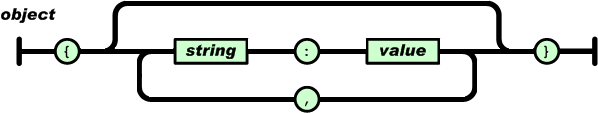
\includegraphics[scale=0.50]{jsondoc.png}
      \caption{Oggetto JSON}
      \label{fig:jsondoc}
  \end{center}
\end{figure}
\\Ogni nome di variabile è seguito dai due punti ``:'' e le coppie
``nome'' : ``valore'' sono separati
da una~virgola~``,''~(Figura~\ref{fig:jsonvalue}).
\begin{figure}[!h]
  \begin{center}
      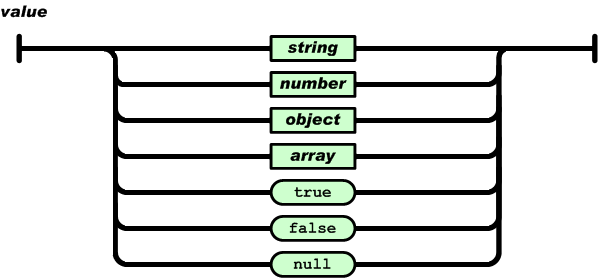
\includegraphics[scale=0.50]{jsonvalue.png}
      \caption{Valore di una variabile JSON}
      \label{fig:jsonvalue}
  \end{center}
\end{figure}
\\Un array è un insieme ordinato di valori. Un array comincia con una parentesi
quadra sinistra ``{[}'' e finisce con una parentesi destra``{]}''. I valori
sono separati da una~virgola~``,''~(Figura~\ref{fig:jsonarray}).
\begin{figure}[!h]
\begin{center}
    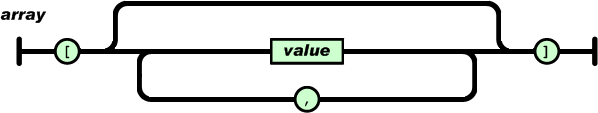
\includegraphics[scale=0.50]{jsonarray.png}
    \caption{Array JSON}
    \label{fig:jsonarray}
\end{center}
\end{figure}
\\\\\\L'oggeto utilizzato nel nostro modello è composto da sei variabili.
\emph{department} indica la facoltà per la quale è stata registrata una
votazione, il valore è una stringa univoca, nel caso la votazione si
riferisca ad un'operazione eseguita presso lo sportello veloce verrà registrata
con \emph{``sportello''}.\emph{Score} è una variabile numerica intera , nel
nostro modello può assumere i valori \{1,3,5\}.La data di effettuazione della
votazione,\emph{date} , viene raccolta dal sistema e salvata nel formato
``Y-m-d''.Gli attributi \emph{comment},\emph{customerName} e
\emph{customerEmail} nel caso il ciente lasci un feedback sono di tipo stringa , \emph{null} altrimenti. 
\\
\begin{lstlisting}[language=json] 
{ 
   _id:"182b00cd54a2b054fffabf1042000fbb", 
   _rev:"1-cb887f197900dce789c2dca898e4d330", 
   department: "engineering",
   score: 5,
   date: "2013-06-01T11:40:52.280Z",
   comment: "Servizio efficiente",
   customerName: "Alex Tomasello",
   customerEmail: null
}
\end{lstlisting} 

\section{Map-Reduce}
\section{Query}

\clearpage{\pagestyle{plain}\cleardoublepage}
\chapter{Promise Pattern}
\label{cha:analisi_framework}
\input{promise.tex}

\clearpage{\pagestyle{plain}\cleardoublepage}
\chapter{Conclusioni}
\label{cha:conclusioni}
\input{conclusioni.tex}

\input{bibliografia.tex}

\end{document}
